\documentclass[12pt]{article}
\usepackage{graphicx}
\usepackage{array}
\pagestyle{empty}

\pdfpagewidth=16in
\pdfpageheight=9in
\setlength{\textwidth}{14.6in}
\setlength{\textheight}{7.6in}
\setlength{\oddsidemargin}{-0.4in}
\setlength{\evensidemargin}{-0.4in}
\setlength{\topmargin}{-0.7in}
\setlength{\parindent}{0pt}
\setlength{\parskip}{0.55em}

\newcommand{\slidetitle}[1]{%
  {\LARGE\bfseries #1}\par
  \vspace{0.2em}\hrule\vspace{0.7em}
}
\newcommand{\twocol}[2]{%
  \begin{minipage}[t]{0.47\textwidth}#1\end{minipage}\hfill
  \begin{minipage}[t]{0.50\textwidth}#2\end{minipage}
}
\newcommand{\newslide}{\clearpage}

\begin{document}

\begin{center}
  \vspace*{1.2in}
  {\Huge\bfseries DSD Final Project}\\[0.4in]
  {\LARGE Pipelined RISC-V Processor Final Submission}\\[0.6in]
  {\Large B12901008 Chung Chia-Yu}\\[0.15in]
  {\Large Group 18}\\[1.0in]
  {\large Final Submission}
\end{center}

\newslide
\slidetitle{Processor Overview}
\twocol{
\begin{itemize}
  \item Five-stage pipelined RISC-V core.
  \item Forwarding and stall units for data hazards.
  \item Branch flush and prediction path.
  \item I-cache and D-cache with slow-memory interface.
\end{itemize}
}{
\begin{itemize}
  \item Supports baseline RV32I required instructions.
  \item Supports compressed instruction fetch/decode.
  \item Supports multiplication instruction pattern.
  \item Cache flush support for final memory check.
\end{itemize}
}

\newslide
\slidetitle{Synthesis Result}
\begin{center}
\begin{tabular}{|l|r|}
\hline
Metric & Value \\
\hline
Clock cycle & 3.00 ns \\
Combinational area & 278998.244294 \\
Noncombinational area & 204061.428898 \\
Buf/Inv area & 38512.308615 \\
Total cell area & 483059.673192 \\
Total area & 4308345.930912 \\
\hline
\end{tabular}
\end{center}

Source: 02-SYN/Report/CHIP-syn.area.

\newslide
\slidetitle{Final Score Summary}
\begin{center}
\begin{tabular}{|l|r|}
\hline
Item & Result \\
\hline
BrPred execution cycles & 526 cycles \\
hasHazard execution cycles & 2235 cycles \\
Compression simulation time & 1990 ns \\
Mul simulation time & 718 ns \\
QSort simulation time & 316447 ns \\
Conv simulation time & 58963 ns \\
LFSR-HIST simulation time & 3250843 ns \\
Performance score & $2.93\times 10^{22}$ \\
\hline
\end{tabular}
\end{center}

\newslide
\slidetitle{Extension: Branch Prediction}
\twocol{
\begin{itemize}
  \item Branch prediction path added before EX resolution.
  \item BTFNT-style direction from branch immediate sign.
  \item Wrong-path instructions are flushed on EX redirect.
\end{itemize}
}{
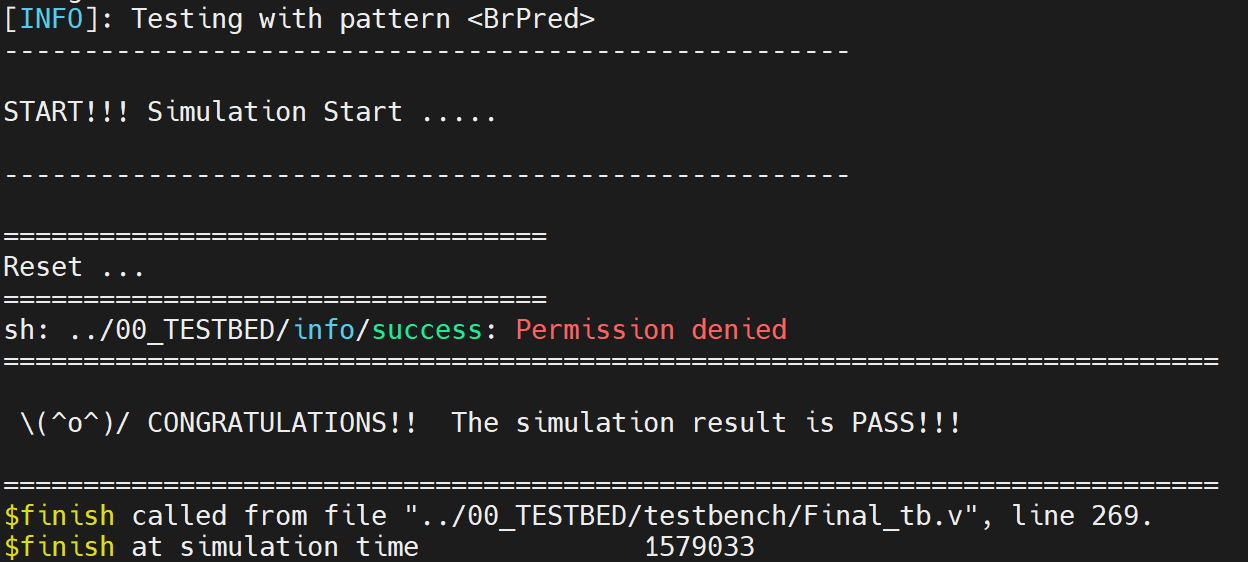
\includegraphics[width=\linewidth]{pic/brpred.png}
}

\newslide
\slidetitle{Extension: Compressed Instructions}
\twocol{
\begin{itemize}
  \item 16-bit instruction length detection in IF.
  \item Decompression into internal 32-bit instruction form.
  \item Handles unaligned 32-bit instruction crossing word boundary.
\end{itemize}
}{
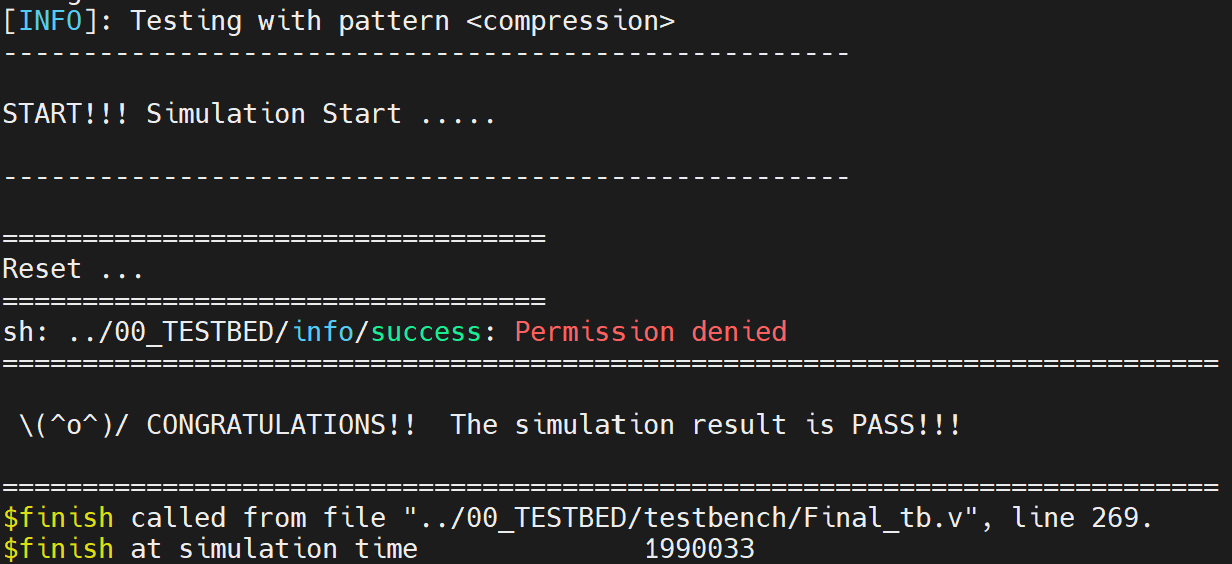
\includegraphics[width=\linewidth]{pic/compression.png}
}

\newslide
\slidetitle{Extension: Multiplication}
\twocol{
\begin{itemize}
  \item Multi-cycle multiplication support.
  \item Pipeline stalls while multiplication result is pending.
  \item Dedicated multiplier state keeps forwarding inputs stable.
\end{itemize}
}{
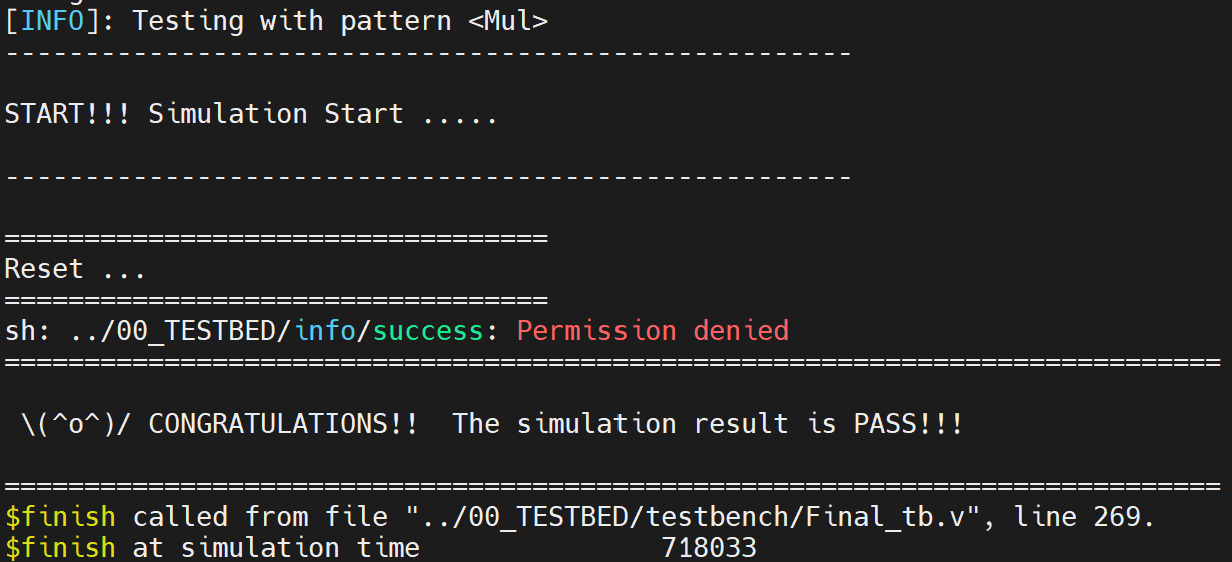
\includegraphics[width=\linewidth]{pic/mul.png}
}

\newslide
\slidetitle{Performance Patterns}
\begin{center}
\begin{tabular}{ccc}
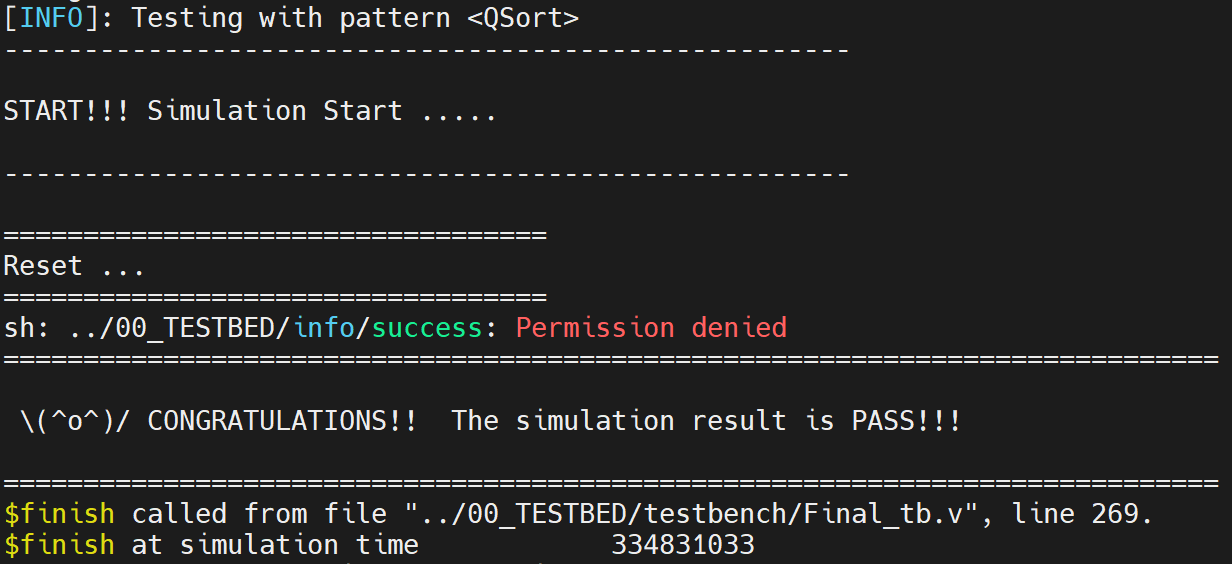
\includegraphics[width=0.30\textwidth]{pic/qsort.png} &
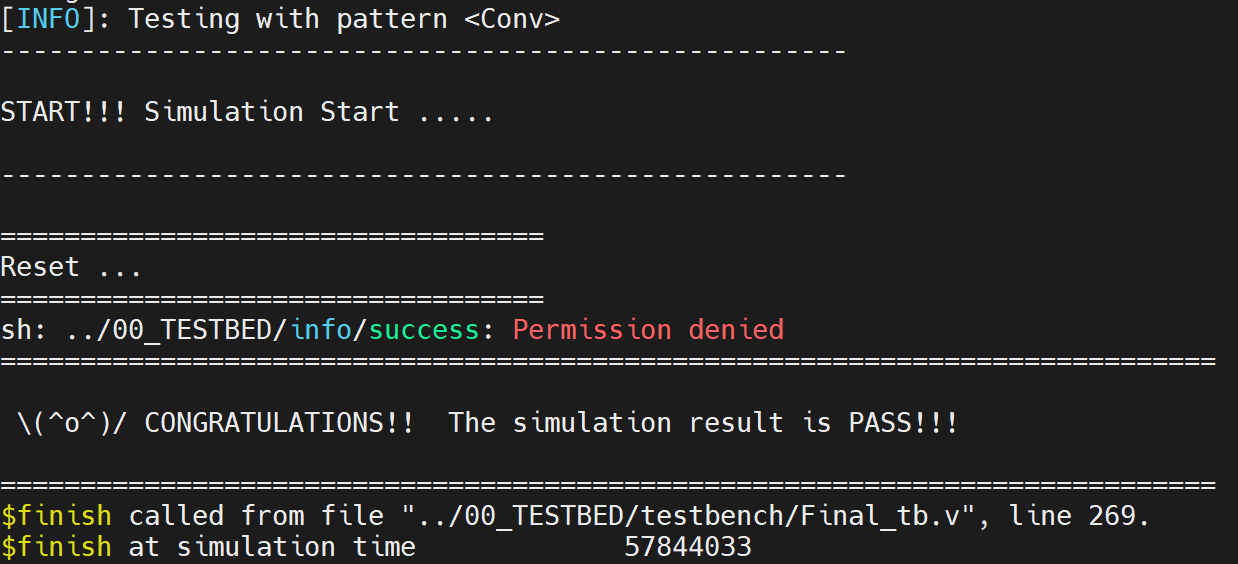
\includegraphics[width=0.30\textwidth]{pic/conv.png} &
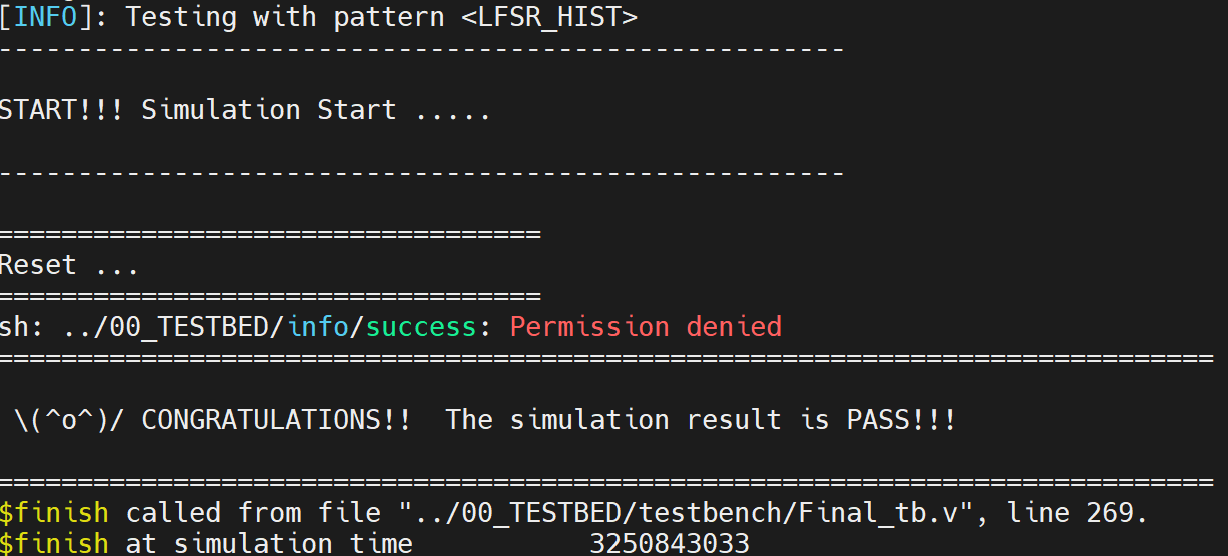
\includegraphics[width=0.30\textwidth]{pic/LFSR_HIST.png} \\
QSort & Conv & LFSR-HIST
\end{tabular}
\end{center}

\newslide
\slidetitle{Cache Sweep Research}
\begin{center}
\begin{tabular}{|l|r|r|r|r|}
\hline
Pattern & Blocks & Ways & Total misses & Expected memory delay (ns) \\
\hline
QSort & 16 & 1 & 1861 & 99945 \\
QSort & 32 & 1 & 387 & 27225 \\
QSort & 32 & 2 & 289 & 19080 \\
QSort & 64 & 2 & 119 & 7020 \\
\hline
Conv & 16 & 1 & 617 & 33435 \\
Conv & 32 & 1 & 103 & 6075 \\
Conv & 32 & 2 & 106 & 5490 \\
Conv & 64 & 2 & 69 & 3105 \\
\hline
LFSR-HIST & 16 & 1 & 43337 & 1967490 \\
LFSR-HIST & 32 & 1 & 593 & 43200 \\
LFSR-HIST & 32 & 2 & 588 & 42795 \\
LFSR-HIST & 64 & 2 & 566 & 40455 \\
\hline
\end{tabular}
\end{center}
Key observation: larger caches reduce miss cost, but high associativity gives limited improvement compared with its timing and area cost.

\newslide
\slidetitle{Branch Predictor Sweep Research}
\begin{center}
\begin{tabular}{|l|r|r|}
\hline
Predictor on BrPred & Accuracy & Storage cost \\
\hline
Always not taken & 37.97\% & 0 FF \\
Always taken & 62.03\% & 0 FF \\
BTFNT & 73.42\% & 0 predictor FF \\
Global 3-bit counter & 68.35\% & 3 FF \\
4-entry gshare 2-bit & 86.08\% & 8 FF + history \\
8-entry bimodal 2-bit & 93.67\% & 16 FF \\
\hline
\end{tabular}
\end{center}
\vspace{0.2in}
\begin{center}
\begin{tabular}{|l|r|r|r|}
\hline
Pattern & Always NT & BTFNT & Global 3-bit \\
\hline
QSort & 72.44\% & 72.44\% & 70.48\% \\
Conv & 63.58\% & 66.05\% & 63.58\% \\
LFSR-HIST & 85.46\% & 85.46\% & 85.44\% \\
\hline
\end{tabular}
\end{center}
Final choice: BTFNT gives a useful BrPred gain with very low hardware cost.

\end{document}


